\newpage
\begin{center}
	This page was intentionally left blank.
\end{center}
\newpage
\chapter{Machine Learning and Collaborative filtering}
\section{Machine Learning} Learning is the complex process that contains among other knowledge acquisition and organization.

\paragraph{}Moving forward lets examine the objectives and processes of machine learning \cite{carbonell1983overview}. The objectives of machine learning can be summarized in three major categories as shown below.

\begin{description}
	\item[$\bullet$ Task Oriented Studies] Those studies emphasize on creating and analyzing a predefined set of tasks in order to improve their performance. They are also called engineering approach.
	\item[$\bullet$ Cognitive Simulation] In this area, the computer program tries to imitate the learning process of a human being.
	\item[$\bullet$ Theoretical Analisis] is the last but not least of the machine learning objectives. Here is where scientists try to investigate, domain agnostic learning processes and algorithms.
\end{description}

\paragraph{} It is stated that there are two types of learning. Those types are knowledge acquisition and skill refinement. To make things more clear let us give some examples. Let us assume that you are studying about a new dog breed. This type of learning will be based on the acquisition of the knowledge. What color usually this breed is, what is its sizes and so on. Now let us assume that is the second time you are riding a bike, you have the knowledge of what goes where but your skill is not refined. As you will continue to ride the bike you will follow the second type of learning which is the skill refinement.

\paragraph{} Numerous processes of learning is known, from processes that someone may call naive, to very efficient and complex ones. Below is listed roughly some of those processes.

\begin{description}
	\item[$\bullet$ Rote learning and direct implanting of knowledge] process requires no knowledge transformation by the learner. The learner deterministically responding the knowledge we put in. When a computer programmer, instructs its machine through the code he provided, and that code contains an if statement. This is a knowledge that has been directly implanted to it.
	\item[$\bullet$ Learning by instruction], for example, we provide a set of rules to a program in a given language. The receiving system or the learner if you prefer, will have to transform this knowledge in order to utilize it.
	\item[$\bullet$ Learning by analogy] is the process that allows the learner to project an existing knowledge to the new one in order to understand it.
	
	
	For example, let us imagine ourselves in an auditorium, and we having a class about lions. In order to help the example, let us assume that the only knowledge we have about the animal kingdom is dogs and cats. The professor knows or at least suspecting the specific knowledge we have. Then he says, a lion has the body structure of a cat and its size is twice as much the dog. We projected the new knowledge on a given one.
	
	\item[$\bullet$ Learning by example.] In this area we give to the learner a set of examples which are notated as true or false. The learner will have to make assumptions and create patterns between the examples in order to answer a request that is not notated.
	
	\item[$\bullet$ Learning from observation and discovery] is the last process we are going to investigate. This process is also called \textit{unsupervised learning}.
	In this type of learning the learner tries to classify the observations without the help of a supervisor. Unsupervised learning has two main aspects. The first aspect is the \underline{passive observation}. In this aspect, the learner classifies the observations made to the environment he exists. The second and more interesting part of is the \underline{active experimentation}. This is where the learner tries to perturb its environment and observe the results of it. 
	
	Let's give an example of active experimentation. Assuming we have a smart virtual machine hypervisor. The hypervisor follows the unsupervised active experimentation learning paradigm. This hypervisor hosts a virtual machine of 5 cores and 2GB of memory. The hypervisor has information about the number of processors used, the amount of memory available to the system and the traffic network.
	
	The hypervisor decides to experiment on the virtual machine and reduces the amount of available memory to 128MB. Instantly the hypervisor observes a dramatic reduction in the network traffic and the memory usage to be 100\%. On the other hand, the 5 cores are underutilized. Those metrics makes the learner classify this situation as a nonregular and returns the resources to the virtual machine.
	
\end{description}

\subsection{Latest advancements in machine learning}
\paragraph{}Nowadays, deep neural networks can win games using strategies that a player could not expect. Like a biological brain, it consists of layers of neurons, but this time is figments of memory. Lower level neurons analyze pixels of a picture then they send data to higher level neurons which are trained on higher level concepts like a dog or a cat. Deep neural networks have shown that they can recognize items on a picture as accurately as humans do.

\paragraph{} In a conference in Berlin has presented evidence in support of a new theory on how deep learning works by a computer scientist and neuroscientist from the Hebrew University of Jerusalem. This man called Naftaly Tishby argues that deep neural networks learn by a process called \textit{information bottle neck} \cite{tishby2000information}. The theory states that the network gets rid of the noise in order to pass information to higher level neurons. A Google researcher, Alexander A. Alemi, states that this theory could serve "not only as a theoretical tool for understanding why our neural networks work as well as the way they do currently, but also as a tool for constructing new objects and architectures".

\section{Collaborative filtering}
\paragraph{} In order to better understand the term, collaborative filtering lets take a look in a dictionary.
\paragraph{collaborative:} adjective, characterized or accomplished by collaboration \cite{Dictionary.com2017}.
\paragraph{filter:} noun, something that works like a filter, as by removing, blocking, or separating out certain elements \cite{Dictionary.com2017}.
\paragraph{} As we can see by the given definitions, collaborative filtering is the technique that allows us to select an object from a given set based on the set itself.
\paragraph{}The need of having recommender systems lies between the need of obtaining recommendations from trustworthy sources and the availability of a large amount of user data.
\paragraph{}Like on any demand and supply system, on the one hand, lies the demand of accurate and trustworthy recommendations. On the other hand are the tons of user data that can serve this demand.
\paragraph{}Over the years have been developed techniques that can utilize those data, in order to provide good recommendations. Those techniques are highly dependent on the volume of data they use. 

\paragraph{}The more the data the more accurate the recommendation. But its system's training phase is largely impacted by the volume mentioned before. Thus, any algorithm or system is will provide good recommendations as long as it is trained with the right dataset.

\paragraph{} Those algorithms were initially based only on statistical models that were available at the time. Whereas the data were growing rapidly, and the sample started to approach the population.
\subsection{Content based}
\paragraph{} Content-based, it seems a very attractive term but let us take a look at the very definition of those words.
\paragraph{content:} noun, something that is contained \cite{Dictionary.com2017}.
\paragraph{base:} noun, a fundamental principle or groundwork; foundation; basis \cite{Dictionary.com2017}.

\paragraph{}Content based collaborative filtering is the technique that allows us to select objects from a given set based on the actual values of its items.
\paragraph{} This could be a rote or information implant learning processes.

\paragraph{}The most common and easy to interpret the way of recommendation is content-based collaborative filtering. In this area of algorithms, you are trying to utilize data from other users in order to come to a recommendation. Those data might be attributes that characterize the item of interest. 
\paragraph{}In the case of users, those attributes may be their age or occupation, whereas for a product might be its color, prize or weight in kilograms. In order to put this to a mathematical expression, we could write the following.

\begin{equation}
w=R^{-1}M^{T}
\end{equation}

\paragraph{}Raw data though are not always clear or normalized. Due to this fact, we would consider to normalizing the approach we used above. If we were about to add a normalization factor to that expression we will end up with the one below.

\begin{equation}
w=(\lambda I + R^{T}R)^{-1} R^{T}M 
\end{equation}

\paragraph{}That kind of algorithms is easier to interpret. They also can handle well a cold-start problem. But they are computational heavy, meaning that the scaling of them is limited.

\subsection{Latent Factors}
\paragraph{} Finally let's take a look at the terms latent and factor in the dictionary.
\paragraph{latent:} adjective present but not visible, apparent, or actualized; existing as potential \cite{Dictionary.com2017}.
\paragraph{factor:} noun one of the elements contributing to a particular result or situation \cite{Dictionary.com2017}.
\paragraph{} Based on the definitions above we can assume that the latent factor collaborative filtering, allows us to select objects from a given set based on factors that are not clearly depicted in the actual values of each item.
\paragraph{} This type of learning is learning by example.
\paragraph{} The group of latent factors algorithms does not take into consideration the meta-data we have for any user or item. 
\paragraph{} In that area, we are trying to determine relationships between a user and an item based only on the rating. Those relationships may not be the age or the color.

\begin{figure}[h]
	\centering
	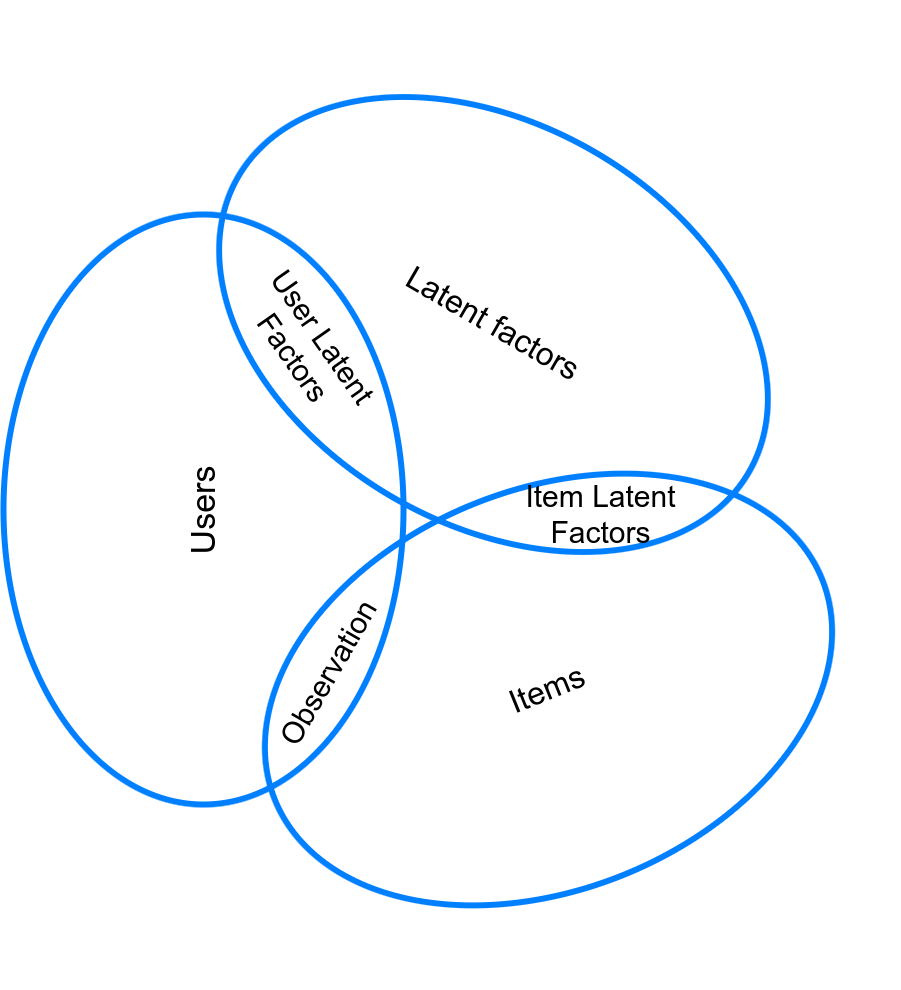
\includegraphics[width=0.5\textwidth]{images/LatentFactors.png}
	\caption{\bfseries LatentFactors}
	\label{LatentFactors}
\end{figure}


\paragraph{} Alternating least squares (ALS) algorithm belongs to the group above. In this case, we assign initially random values of rating between user and items. Then it takes the error between the actual value and the one assigned to it. 

\paragraph{}Then the algorithm runs again using as input the errors and tries to minimize them. Below we can see a how this algorithm is defined. \\

\begin{algorithm}
	\caption{ALS for Matrix Completion}\label{ALS}
	\begin{algorithmic}[1]
		\State Initialize X,Y
		\Repeat
		\For{\texttt{u=1...n}}
		\State $x_{u} = (\sum_{r_{ui}}y_{i}y_{i}^{T} + \lambda I_k)^{-1} \sum_{r_{ui}}r_{ui}y_{i} ,\in r_{u*}$
		\EndFor
		\For{\texttt{i=1...m}}
		\State $y_{i} = (\sum_{r_{ui}}x_{u}x_{u}^{T} + \lambda I_k)^{-1} \sum_{r_{ui}}r_{ui}x_{u} ,\in r_{*i}$
		\EndFor
		\Until {convergence}
	\end{algorithmic}
\end{algorithm}

\paragraph{}As we can see above, this algorithm has a $\lambda$ parameter used for normalization during the process. We can see the difference below where we have both the expression with and without normalization factor.

\paragraph{} ALS is a very efficient recommender algorithm. Due to its nature, it can be easily parallelized reducing the execution time needed \cite{DistributedAlgorithmsAndOptimization:4}. It also requires no meta-data about any user or item. Although, ALS suffers from the cold start problem.

\begin{equation}
\min_{X,Y} \sum_{r_{ui}observed}(r_{ui}-x_{u}^{T}y_{i})^{2}
\end{equation}

\begin{equation}
\min_{X,Y} \sum_{r_{ui}observed}(r_{ui}-x_{u}^{T}y_{i})^{2} + \lambda(\sum_{u}||x_{u}||^2 + \sum_{i}||y_{i}||^2)
\end{equation}

\paragraph{} Moving forward this thesis, we are going to discuss how those two algorithms were implemented and validate the results they gave.